\begin{align}
		\vec{n} = \myvec{
	  12 \\
	  -5 
	  } ,   c = -82 
	  \\
	  \implies 
	d 
	= \frac{\abs{  \myvec{12 & -5 }\myvec{-1 \\ 1}-\brak{-82} }}{\sqrt{12^2+\brak{-5}^2}} 	
	= 5
\end{align}
\iffalse
See \figref{fig:11/10/3/4/Fig1}.
\begin{figure}[H]
	\begin{center}
		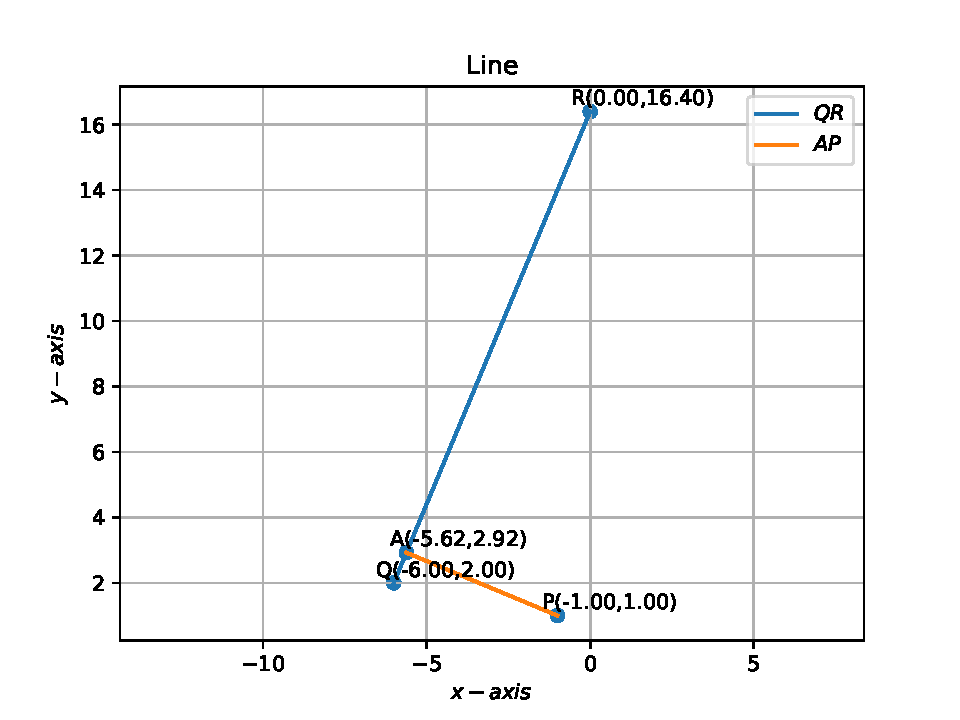
\includegraphics[width=0.75\columnwidth]{chapters/11/10/3/4/figs/problem4.pdf}
	\end{center}
\caption{}
\label{fig:11/10/3/4/Fig1}
\end{figure}
\fi
